
% --------------------------------
% studies, performance
%-----
%\section{Strang Splitting}
%-----
\section{Performance Studies with OpenCMISS Iron}

\iffalse
Next, we study the performance of the software by evaluating runtimes and parallel scalability for different solvers.
We begin with OpenCMISS Iron as the baseline solver that also implements parts of the multi-scale model considered in this work. The work of \cite{Heidlauf2013} describes the implementation of the fiber based electrophysiology model coupled to a quasi-static hyperelastic material model with OpenCMISS. The implementation is parallelized for a hardcoded number of four processes and serves as the baseline code for the following studies.

We improved the performance of this solver for the multi-scale model by two actions: First, we evaluated and optimized the employed numeric schemes. Second, we implemented parallel partitioning for an arbitrary number of processes and evaluated different parallelization strategies.
These changes were directly implemented in the OpenCMISS code. The improvements were also presented in a publication \cite{Bradley:2018:EDB}. In the following sections \cref{sec:opencmiss_numeric_improvements,sec:opencmiss_parallel_partitioning}, we describe the numeric improvements and the parallel partitioning strategies. In \cref{sec:opencmiss_memory}, we discuss the parallel weak scaling and memory consumption properties.

\subsection{Numeric Improvements}\label{sec:opencmiss_numeric_improvements}

The first numeric improvement is to replace the GMRES solver that is used to solve the 1D electric conduction problem on the muscle fibers
by a faster direct solver. 

As noted in \cref{sec:improved_parallel_solver_for_fiber_based}, the 1D electric conduction problem of the monodomain equation yields a tridiagonal system that can be solved with linear time complexity. The baseline solver code employs the restarted GMRES solver of PETSc, which is the default linear system solver in OpenCMISS Iron, as it is a robust choice for abitrary system matrices. 
More efficient solvers exist for symmetric positive definite systems such as the conjugate gradient scheme. 
Furthermore, the MUMPS package \cite{mumps2001} that can be interfaced in PETSc provides a parallel implementation of a direct, multi-frontal linear solver, which is able to exploit banded structures of the system matrix.

We study the runtime of these three solvers for different problem sizes of the 1D problem. The monodomain equation is solved on a single muscle fiber and the number of 1D elements is varied from 15 to 2807. The used timestep widths are $\dt_\text{0D}=\SI{1e-4}{\ms}$ and $\dt_\text{1D}=\SI{5e-3}{\ms}$. The end time of the simulation is $\SI{3}{\ms}$, yielding a total number of 600 solutions of the linear system. The study is executed on an Intel Xeon E7540 processor with 24 cores, clock frequency of \SI{1064}{\mega\hertz} and \SI{506}{\gibi\byte} RAM.

\Cref{fig:opencmiss_linear_solvers} shows the runtime of the GMRES, conjugate gradient and direct solvers for this problem in a double-logarithmic plot.
It can be seen, that, for coarse discretizations with a low number of 1D elements per fiber, the GMRES and conjugate gradient solvers are faster than the direct solver. For finer discretizations, the conjugate gradient solver and the direct solver outperform the GMRES solver. For fibers with more than approximately 500 elements, the direct solver has the lowest runtime. Moreover, the direct solver exhibits an almost linear runtime complexity in terms of the problem size. This indicates that the solver is able to exploit the tridiagonal structure of the system matrix.

% linear solvers plot
\begin{figure}
  \centering%
  \includegraphics[width=0.9\textwidth]{images/results/studies/opencmiss_linear_solvers.pdf}%
  \caption{Numeric improvements in OpenCMISS: Runtime evaluation of different linear system solvers for a single muscle fiber with varying spatial resolution.}%
  \label{fig:opencmiss_linear_solvers}%
\end{figure}%

The second numeric improvement is the exchange of first-order accurate timestepping schemes by second-order schemes. For this exchange, we implemented the Strang operator splitting scheme and use it with the existing Crank-Nicolson implementation in OpenCMISS Iron and the Heun method, which was  implemented by Aaron Krämer.

Numerical studies by Aaron Krämer presented in \cite{Bradley:2018:EDB} show that the relation $K=\dt_\text{1D}/\dt_\text{0D}$ between the timestep width $\dt_\text{1D}$ of the 1D electric conduction problem and the timestep width $\dt_\text{0D}$ of the 0D subcellular model has to be set to $K=2$ and $K=5$ for the Godunov and Strang splitting schemes, respectively, such that the errors of the 0D and 1D subproblems are balanced. To achieve a total error for the membrane potential $V_m$ of approximately \num{8e-2}, we can increase the required splitting timestep width $\dt_\text{splitting}$ from $\SI{5e-4}{\ms}$ for the Godunov splitting to $\SI{4e-3}{\ms}$ for the Strang splitting scheme. This results in a runtime speedup  of approximately 7.5.

To evaluate the total speedup of the described numeric improvements, we compare the runtimes without and with the improvements for a complete simulation of the fiber based electrophysiology model coupled with the elasticity model. A cuboid 3D domain is discretized by $2\times 2\times 2=8$ finite elements for the elasticity model and embeds $6\times 6=36$ 1D fiber meshes. The number of 1D elements per fiber is varied between 576 and \num{239400} to study the scaling behavior of the solvers depending on the problem size. The problem is solved in serial to avoid effects introduced by the parallelization.

The baseline implementation uses the Godunov splitting with forward and implicit Euler schemes for the 0D subcellular model and the electric conduction model, respectively. The linear system in the 1D problem is solved by a GMRES solver with relative residuum tolerance of \num{1e-5} and restart after 30 iterations. Timestep widths of $\dt_\text{0D}=\SI{1e-4}{\ms}$ and $\dt_\text{splitting}=\dt_\text{1D}=\SI{5e-4}{\ms}$ are used. The improved scheme uses the Strang operator splitting with Heun and Crank-Nicolson schemes and timestep widths of $\dt_\text{0D}=\SI{2e-3}{\ms}$ and $\dt_\text{splitting}=\dt_\text{1D} = \SI{4e-3}{\ms}$. The direct solver is used for the linear system in the 1D problem.
The solver for the 3D elasticity problem is the same for both implementations. A Newton scheme with residual tolerance of \num{1e-8} is used
 and coupled to the 0D and 1D solvers with a coupling timestep width of $\dt_\text{3D}=\SI{1}{\ms}$.

The present study and the studies in the next section are executed on the supercomputer \emph{Hazel Hen} at the High Performance Computing Center Stuttgart. This Cray XC40 system contains compute nodes with two Intel Haswell E5-2680v3 processors with a base frequency of \SI{2.5}{\giga\hertz}, 12 cores per CPU, 24 cores per compute node and \SI{128}{\giga\byte} RAM per node.

% improvements plot
\begin{figure}
  \centering%
  \includegraphics[width=\textwidth]{images/results/studies/opencmiss_cuboid_serial_scaling_comparison_aggressive.pdf}%
  \caption{Numeric improvements in OpenCMISS: Study to evaluate the speedup of the improved implementation of the fiber-based electrophysiology and mechanics model in OpenCMISS.}%
  \label{fig:opencmiss_improvements}%
\end{figure}%
% 576.0, 792.0, 1224.0, 1872.0, 2736.0, 4176.0, 6192.0, 9360.0, 14040.0, 21024.0, 31536.0, 47304.0, 70920.0, 106416.0, 159624.0, 239400.0

\Cref{fig:opencmiss_improvements} shows the results of this study. In the upper part, the runtimes for different components of the simulation are indicated by different colors in a plot with double logarithmic scale. The runtimes for the baseline implementation are shown by solid lines and the runtimes including the improvements are shown by dashed lines. In the lower plot, the speedups from the baseline to the improved implementation are given.

The total runtime of the simulation is given by the black lines in the upper plot. It can be seen that the total runtime results almost completely from the 0D model solver, which is shown by the yellow lines. The 1D solver, given by the red lines, has the second most influence. The effects of the data mapping operations between the 3D mesh and the 1D fibers on the runtime are negligible. These data mapping operations consists of the homogenization step from the 1D fibers to the 3D mesh and the interpolation step from the 3D mesh to the 1D fibers.

The runtimes for almost all problem parts increase linearly for increasing mesh resolution of the 1D fibers. Only the runtime of the 3D problem stays constant, as the 3D mesh is unchanged for the different runs.

Significant runtime improvements of the new implementation compared to the baseline implementation can be seen in the lower plot of   \cref{fig:opencmiss_improvements} for the 0D solver and the 1D solver. The speedup for the 0D solver is constant at approximately 2.5. The speedup resulting from the improved linear system solver in the 1D problem is approximately 6.1 for coarse meshes and increases to 14.7 for the finest mesh. This increase for high mesh resolutions results from the higher runtime of the GMRES solver for large problem sizes in the baseline implementation. The overall speedup is similar to the speedup of the 0D problem, as the 0D solver is responsible for the most runtime of the computation.

This study shows how numeric investigations can help to reduce the total runtime, in this case by a factor of 2.5. Moreover, the solver of the 0D model has the most potential to further speed up computation times.

\subsection{Parallel Partitioning Strategies}\label{sec:opencmiss_parallel_partitioning}

To exploit parallelism and, thus, further reduce the computation times, we implemented a generic domain decomposition for the studied problem in OpenCMISS Iron.
Like in OpenDiHu, the 3D mesh can be partitioned to an arbitrary number of $n_x \times n_y \times n_z$ subdomains. The embedded 1D fibers are aligned with the $z$ axis and are partitioned by the same cut planes as the 3D mesh.

% pillars-cubes visualization
\begin{figure}[H]
  \centering%
  \begin{subfigure}[t]{0.48\textwidth}%
    \centering%
    \def\svgwidth{0.7\textwidth}
    \input{images/results/studies/opencmiss_ddpillar.pdf_tex}%
    \caption{\say{Pillar-like} domain decomposition with $n_z=1$.}%
    \label{fig:opencmiss_ddpillar}%
  \end{subfigure}
  \quad
  \begin{subfigure}[t]{0.48\textwidth}%
    \centering%
    \def\svgwidth{0.7\textwidth}
    \input{images/results/studies/opencmiss_ddcube.pdf_tex}%
    \caption{\say{Cube-like} domain decomposition}%
    \label{fig:opencmiss_ddcube}%
  \end{subfigure}   
  \caption{Different parallelization strategies that are implemented in the OpenCMISS model. This figure shows two approaches how the domain can be partitioned to 16 subdomains.}%
  \label{fig:opencmiss_dd_annotated}%
\end{figure}%

\Cref{fig:opencmiss_dd_annotated} shows two exemplary partitionings. If the domain is only partitioned in $x$ and $y$ directions, the fibers are not split into multiple subdomains. As a result, we get \say{pillar} subdomains as shown in \cref{fig:opencmiss_ddpillar}. An alternative approach is to subdivide the domain in all three coordinate directions such that the subdomains are approximately cube shaped, as shown in \cref{fig:opencmiss_ddcube}.

OpenCMISS Iron already provides the functionality to create partitioned unstructured meshes. However, every mesh has to be partitioned into non-empty subdomains for all processes. Thus, it is not possible to use individual meshes for the 1D fibers.
In the baseline implementation of the model by \cite{Heidlauf2013}, all 1D fiber meshes are instead realized as a single mesh, whose node positions are set according to the positions of the individual fibers. This facilitates the implementation of the 0D subcellular model solvers and 1D model solvers, as the implementation has to deal with only a single mesh. 

To allow for an arbitrary partitioning as in \cref{fig:opencmiss_dd_annotated}, we assigned the 1D elements of the single fiber mesh to the same processes as the subdomains of the 3D mesh. Furthermore, we reimplemented the data mapping between the 1D mesh and the 3D mesh, which was hardcoded for four processes.

In the following, we investigate the effect of different partitioning strategies on the overall runtime of the solver. The idea is that, for pillar-like partitionings as in \cref{fig:opencmiss_ddpillar}, the 1D problems could potentially be solved faster, as the fibers, which are aligned in $z$-direction, are not subdivided to multiple processes. On the other hand, the partitioning to cubes in \cref{fig:opencmiss_ddcube} requires less communication in the solution of the 3D problem as the cubes minimize the surface of each subdomain and, in consequence, the amount of data to be exchanged. We evaluate how these effects influence the runtime for the pillar-like partitioning, the cube partitioning and all other possible partitionings specified by numbers of subdomains $n_x \times n_y \times n_z$.

Our test case uses a 3D mesh with $12 \times 12 \times 144$ elements. To reduce the runtime contribution of the 0D/1D electrophysiology problem and the memory consumption of the solver, only two 1D elements per 3D element are included. The numeric parameters are the same as for the improved scenario presented in \cref{fig:opencmiss_improvements}. The simulations are executed on 12 compute nodes of the supercomputer Hazel Hen with 12 processes per node.

We partition the 3D domain to 144 processes using different combinations of $n_x,n_y$ and $n_z$ such that $n_x\,n_y\,n_z=144$. 
For every partitioning, we compute the average surface area of the boundary of every subdomain. 
\Cref{fig:opencmiss_partition_shape} shows the resulting runtime in relation to this average boundary area.
The pillar-like partitioning uses $12 \times 12 \times 1$ subdomains and exhibits the largest boundary surface area, corresponding to the last point in \cref{fig:opencmiss_partition_shape}. The cube partitioning consists of $6 \times 6 \times 4$ subdomains and corresponds to the first data point with the smallest boundary area.

% plot of partition shapes
\begin{figure}
  \centering%
  \includegraphics[width=\textwidth]{images/results/studies/opencmiss_partition_shape.png}%
  \caption{Runtime of the solvers for different partition shapes, from cube partitions on the left to pillar partitions on the right.  \footnotesize(This figure has also been published in \cite{Bradley:2018:EDB} under a creative commons license.)}%
  \label{fig:opencmiss_partition_shape}%
\end{figure}%

The plot shows that the runtime of the 3D solver increases approximately linearly with the amount of communication, which is expected.
The partitioning with the largest average surface area has a runtime that is approximately four times as large as the runtime for the smallest surface area.

Moreover, the plot shows that the partitioning scheme has no significant influence on the runtime of the 1D solver. The reason is that the implementation does not fully reflect the decoupled nature of the individual problems of the fibers. As noted before, one big linear system has to be solved that contains the degrees of freedom of all fibers. The degrees of freedom are ordered by PETSc such that the nodes within every subdomain are consecutive. If a subdomain contains (parts of) multiple fibers, their degrees of freedom are not necessarily consecutive in the solution vector and communication is required.

\subsection{Weak Scaling Study and Memory Consumption}\label{sec:opencmiss_memory}

Next, we evaluate the parallel weak scaling properties of the overall solver. We increase the number of elements in the 3D mesh from 1232 to 8640 and the total number of 1D elements in all fibers from \num{14784} to \num{103680}. Correspondingly, the number of processes increases from 24 to 192, such that the amount of work per process stays approximately constant. Each scenario is computed with two different partitioning schemes, once with a pillar-like partitioning and once with a cube partitioning. For the exact problem sizes, numbers of cores and numbers of elements in the partitions, we refer to the paper \cite{Bradley:2018:EDB}. 

% weak scaling runtime
\begin{figure}
  \centering%
  \includegraphics[width=\textwidth]{images/results/studies/opencmiss_weak_scaling.png}%
  \caption{Parallel weak scaling study of a scenario with the pillars and cubes partitionings.  \footnotesize(This figure has also been published in \cite{Bradley:2018:EDB} under a creative commons license.)}%
  \label{fig:opencmiss_weak_scaling}%
\end{figure}

\Cref{fig:opencmiss_weak_scaling} shows the resulting runtimes of the different components of the simulation. It can be seen that the runtime stays approximately the same for all problem sizes. The observable differences in runtime within the same solver, especially for the last two data points, can be explained by a slighly different ratio of element count to process count, which results from the goal to use the pillar and cubes partitioning schemes while not exceeding the available main memory.

The runtimes of the pillars and cubes partitioning schemes are depicted by dashed and solid lines, respectively. The pillars partitioning exhibits shorter runtimes for the 1D solver and longer runtimes for the 3D solver compared to the cubes partitioning. In total, the runtime is not significantly different for the different partitioning strategies.

% memory consumption
\begin{figure}
  \centering%
  \includegraphics[width=\textwidth]{images/results/studies/opencmiss_memory.png}%
  \caption{Memory consumption per process at the end of the simulation corresponding to the weak scaling study of \cref{fig:opencmiss_weak_scaling}. \footnotesize(This figure has also been published in \cite{Bradley:2018:EDB} under a creative commons license.)}%
  \label{fig:opencmiss_memory}%
\end{figure}%

A limiting factor for the construction of weak scaling studies with this implementation is the high memory consumption. \Cref{fig:opencmiss_memory} shows the total memory consumption per process at the end of the runtime of the simulations in \cref{fig:opencmiss_weak_scaling}. The used memory is visualized by purple lines. The dashed line again corresponds to the pillars partitioning and the solid line corresponds to the cubes partitioning. 

As can be seen, the memory consumption per process monotonically increases with the total number of 1D elements. 
At the same time, however, the number of elements per process stays approximately constant in this weak scaling setting. The last data point is close to the memory limit of $\SI{128}{\giga\byte} / 24 \approx \SI{4.967}{\gibi\byte}$, which is reached when 24 processes are executed on a compute node of the supercomputer Hazel Hen.

A difference between the pillar partitions and the cube partitions is the size of the subdomain surfaces and the corresponding size of the ghost layer. \cref{fig:opencmiss_memory} shows the number of 3D ghost elements for the scenarios with cubes and pillars by the black lines. In OpenCMISS, a ghost element on a process is an element that contains ghost nodes, which are owned by a different process. The ghost elements serve as data buffers for communication during the assembly of the finite element matrices, similar to OpenDiHu.

The plot in \cref{fig:opencmiss_memory} shows that the number of ghost elements is higher for the pillar partitioning scheme than for the cubes scheme, as expected. In consequence, the memory consumption per process is also slightly higher for the pillar partitioning.
However, this effect is negligible compared to the high absolute value of the required memory and does not explain this effect.

The increase in memory results from the organization of parallel partitioned data in OpenCMISS Iron. On every process, global mesh topology information such as mappings between global indexing and local indexing is stored for the element numbers, node numbers and degree of freedom numbers. While this overhead in storage is negligible for moderately parallel scenarios, it counteracts the domain decomposition approach for higher degrees of parallelism. 

Numerous functions and algorithms in the OpenCMISS Iron code rely on this type of global information. Thus, eliminating the parallelism constraint by reorganizing the data structures is a highly involved task. Especially the initialization of the parallel partitioning heavily uses this global information. This initialization includes, e.g., the distribution of elements and nodes to the subdomains on the processes, the determination of the ghost layers and dofs to send to and receive from neighbor processes, and the setup of local numbers for elements, nodes and degrees of freedom.

We addressed the elimination of this use of global topology information in the initialization steps and developed and implemented appropriate local algorithms in OpenCMISS Iron. This resulted in major code changes that are difficult to oversee, also because of the lacking object orientation in the code base and the difficulty to test the functionality. Creating the required comprehensive set of unit tests for nearly all functionality of OpenCMISS would be a large task that remains to be done. Thus, these code changes could not be merged into the main trunk of OpenCMISS.

Even with these code changes, the memory problem is not yet solved. Another problem prior to the initialization step is that the mesh has to be specified from the user code in a global data structure. It is currently not possible to specify a mesh in a distributed way. Thus, OpenCMISS Iron can only use meshes that initially fit into the main memory on a single core.

Moreover, another issue is concerned with the data structures for matrices. Each process stores its local row indices and additionally a map from global to local row indices for all dofs of the global problem. This global-to-local map also contributes to the bad weak memory scaling and has to be eliminated as well. One possible approach is to use hash maps and only store the relevant portion of the mapping on every process. Work towards resolving this issue has been started by Lorenzo Zanon at the former SimTech Research Group on Continuum Biomechanics and Mechanobiology at the University of Stuttgart. 

One reason for the generic mapping of matrix rows, which uses global information, is that OpenCMISS Iron does not restrict discretization schemes to the finite element method, where the system matrix can be assembled from local element matrices within the subdomains. An example for a different scheme is the boundary element method.

In addition, there exist more parts in the code that use a similar global-to-local mapping and would also have to be changed to allow for a constant memory consumption per process, e.g, the boundary condition handling and the data mapping between the 3D mesh and the fibers.

In summary, fixing the issue of non-scaling memory consumption in OpenCMISS Iron corresponds to redeveloping a significant portion of the code. 
To preserve the generic functionality of OpenCMISS, some changes would require new algorithmic considerations and complex workarounds.
This development effort would have to be quick enough to keep up with the independent development of the normal OpenCMISS branch. After completion, the merge back into the main software trunk would only be possible if the branches had not diverged too far and after significant efforts have been put into testing and preserving the feature set of OpenCMISS.

On the other hand, developing the missing functionality from scratch and making sensible restrictions on the generality of the solved problems and used methods requires possibly less effort and allows to consider design goals such as performance, usability and extensibility from the beginning.
In this sense, the OpenDiHu software project can be seen as a complement to OpenCMISS Iron.  %companion
The mentioned restrictions are, e.g., the exclusive use of the finite element method and cartesian coordinates and the use of parallel partitioned structured meshes instead of the more complex parallelization of unstructured meshes.

%-----

\fi

\section{Evaluation of Compiler Optimizations}

At first, we investigate the auto-vectorization performance of the GNU, Intel
and Cray compilers, and vary optimization levels both for the program and
in the CellmlAdapter. We compute the system of Eqns. (1) and (2) with the
subcellular model of Shorten et al. [18] for one muscle fiber with np = 2400
nodes, time step widths dt0D = 10−3 ms, dt1D = dtsplitting = 3 · 10−3ms and
end time t = 20ms. 24 processes are used on one compute node of Hazel Hen.
The total runtimes for the 0D and 1D parts are depicted in Fig. 5.

The performance measurements are carried out on the supercomputer
Hazel Hen at HLRS in Stuttgart. Per compute node, it contains two Intel
Haswell E5-2680v3 CPUs at 2.5 GHz with 24 cores.

It can be seen, that for all compilers computation times for the 0D model
decrease if the optimization level is increased from O1 to O2 or O3 and further
to Ofast. The optimization levels O2 and O3 behave similarly for the given
program. This shows that vectorization, which is already enabled by the O2
flag, contributes most to the decrease in runtimes. For the same reason, the
computation of the 1D model does not profit from a higher optimization level
of the compiler. When using Ofast, compliance regarding the IEEE and ISO
rules for floating-point arithmetic and math functions gets disregarded, which
means for example that infinite math is not supported. This is not an issue
for our simulation code. As can be seen in the measurement of the GNU and
Intel compilers, this optimization level yields a further increase in performance
with more than 2 times faster code for the GNU compiler. Comparing the
compilers, it can be seen, that, for the same optimization level, the Cray
compiler produces faster code than the Intel compiler, which in turn produces
faster code than the GNU compiler. The best result is achieved with the Cray
compiler and the O3 flag. However, the compile time increases to over 2 hours
compared to approximately 10 minutes with the other two compilers.


% fibers_emg performance
\begin{figure}
  \centering%
  \includegraphics[width=0.7\textwidth]{images/results/studies/compilers.pdf}%
  \caption{Comparison of compilers. Runtime of the 0D and 1D solvers in the fiber based electrophysiology model with \code{simd} optimization type for different compilers and optimization flags.}%
  \label{fig:compilers}%
\end{figure}%
                            %nproc  solve_0D  solve_1D   write    comp.  usertime  overhead    n  memRSS unit
%cray_O2_n24                    24    10.288    11.825  28.525   49.420    47.461  -1.21910  120  57.207  MiB
%cray_O3_n24                    24    10.299    11.787  30.532   48.003    47.681  -4.61410  120  57.137  MiB
%cray_O3_nolib_n24              24    10.252    11.840  24.286   46.265    45.794  -0.11311  120  57.244  MiB
%gnu_O1_n24                     24   261.950    15.817  24.957  311.130   307.120   8.40630  120  54.292  MiB
%gnu_O2_march_native_n24        24    62.553    15.065  25.294  110.650   106.580   7.74220  120  53.822  MiB
%gnu_O2_n24                     24    63.020    15.122  32.335  117.460   108.750   6.98280  216  55.062  MiB
%gnu_O3_march_native_n24        24    63.231    15.633  24.814  109.960   107.620   6.27740  144  54.201  MiB
%gnu_O3_n24                     24    63.228    15.343  31.023  117.290   108.280   7.69120  120  53.724  MiB
%gnu_Ofast_march_native_n24     24    13.583    14.212  29.835   59.794    58.708   2.16380  120  54.165  MiB
%gnu_Ofast_n24                  24    13.580    14.393  33.702   64.771    60.167   3.09660  120  54.074  MiB
%intel_O1_n24                   24    73.255    17.172  27.525  125.280   121.470   7.33120   96  56.213  MiB
%intel_O2_n24                   24    22.894    14.632  30.846   73.070    76.631   4.69830  120  56.337  MiB
%intel_O3_ipo_n24               24    22.913    14.950  26.153   68.646    76.098   4.63060  120  56.534  MiB
%intel_O3_ipo_xHost_n24         24    22.906    14.840  27.502   69.987    76.459   4.73920  120  56.520  MiB
%intel_O3_n24                   24    22.921    14.628  33.568   72.243    76.021   1.12550  120  56.342  MiB
%intel_Ofast_ipo_n24            24    14.292    14.875  29.073   61.534    69.153   3.29290  120  56.347  MiB
%intel_Ofast_ipo_xHost_n24      24    14.339    14.983  25.068   61.882    69.375   7.49200  120  56.493  MiB
%intel_Ofast_n24                24    14.291    14.619  33.398   65.989    70.719   3.68130  120  56.236  MiB


\section{Monodomain Solver Performance}

% fibers_emg performance
\begin{figure}
  \centering%
  \includegraphics[width=\textwidth]{images/results/studies/fibers_emg_study.pdf}%
  \caption{Efficiency model}%
  \label{fig:fibers_emg_study}%
\end{figure}%

% fibers_emg performance shorten
\begin{figure}
  \centering%
  \includegraphics[width=\textwidth]{images/results/studies/fibers_emg_study_shorten.pdf}%
  \caption{Efficiency model shorten}%
  \label{fig:fibers_emg_study_shorten}%
\end{figure}%

% 0/18 : This is opendihu 1.2, built Apr  9 2021, C++ 201703, GCC 10.2.0, current time: 2021/4/9 17:15:06, hostname: pcsgs05, n ranks: 18                                                       
% 0/18 : Open MPI v3.1.6, package: Open MPI maierbn@sgscl1 Distribution, ident: 3.1.6, repo rev: v3.1.6, Mar 18, 2020                                                                           
% 0/18 : File "../settings_fibers_emg.py" loaded.                                                                                                                                               
% 0/18 : ---------------------------------------- begin python output ----------------------------------------                                                                                  
% Loading variables from "ramp_emg.py".                                                                                                                                                         
% scenario_name: fast-vc,  n_subdomains: 3 2 3,  n_ranks: 18,  end_time: 10.0
% dt_0D:           3.0e-03, diffusion_solver_type:      cg                                                                                                                                      
% dt_1D:           1.0e-03, potential_flow_solver_type: gmres, approx. exp.: False                                                                                                              
% dt_splitting:    3.0e-03, emg_solver_type:            cg, emg_initial_guess_nonzero: False                                                                                                    
% dt_3D:           4.0e-01, paraview_output: True, optimization_type: vc (AoVS)                                                                                                                 
% output_timestep: 4.0e+05, surface: 1.0e+00, stimulation_frequency: 0.1 1/ms = 100.0 Hz                                                                                                        
%                           fast_monodomain_solver_optimizations: False                          
% fiber_file:              ../../../input/left_biceps_brachii_25x25fibers.bin                                                                                                                   
% cellml_file:             /data/scratch/maierbn/opendihu/examples/electrophysiology/input/hodgkin_huxley_1952.c                                                                                
% fiber_distribution_file: /data/scratch/maierbn/opendihu/examples/electrophysiology/input/MU_fibre_distribution_10MUs.txt                                                                      
% firing_times_file:       /data/scratch/maierbn/opendihu/examples/electrophysiology/input/MU_firing_times_always.txt                                                                           
% ********************************************************************************                                                                                                              
% prefactor: sigma_eff/(Am*Cm) = 0.03079310344827586 = 8.93 / (500.0*0.58)                                                                                                                      
% diffusion solver type: cg                                                                                                                                                                     
% n fibers:              625 (25 x 25), sampled by stride 2 x 2                                  
% n points per fiber:    1481, sampled by stride 50                                                                                                                                             
% 18 ranks, partitioning: x3 x y2 x z3                                                                                                                                                          
% 25 x 25 = 625 fibers, per partition: 8 x 12 = 96                                                                                                                                              
% per fiber: 1D mesh    nodes global: 1481, local: 500                                           
%   sampling 3D mesh with stride 2 x 2 x 50                                                      
%     linear 3D mesh    nodes global: 13 x 13 x 31 = 5239, local: 4 x 6 x 10 = 240               
%     linear 3D mesh elements global: 12 x 12 x 30 = 4320, local: 4 x 6 x 10 = 240               
% number of degrees of freedom:                                                                  
%                     1D fiber:       1481  (per process: 500)                                   
%             0D-1D monodomain:       5924  (per process: 2000)                                  
%  all fibers 0D-1D monodomain:    3702500  (per process: 192000)                                                                                                                               
%                  3D bidomain:       5239  (per process: 240)                                   
%                        total:    3707739  (per process: 192240)                                                                                                                               
% Python config parsed in 0.1s.        
% 0/18 : ----------------------------------------- end python output -----------------------------------------                                                                                  
% 0/18 : Read from file "../../../input/left_biceps_brachii_25x25fibers.bin", 502 collective chunks.                                                                                            
% done.                                                              

% plot:
%------------------------------------------------------------------------------------------------------------------------
%logs/log_optimization_type_study.csv
                     %subdomains         user  total comp.          0D          1D   bidomain  duration_init  write       mem    n
%scenarioName  nRanks                                                                                                             
%fast-gpu      1       [1, 1, 1]   400.990000   396.361500         NaN         NaN   0.289390       4.628500    0.0  1.553 GB    2
%fast-vc       18      [3, 2, 3]    47.087778    43.088483   33.531100    1.575581   2.215858       3.999294    0.0  0.200 GB   36
%fast-vc-apx-e 18      [3, 2, 3]    20.227431    15.370216    8.867359    1.937768   1.158790       4.857215    0.0  0.200 GB  144
%openmp-18-0   18      [3, 2, 3]   235.358889   233.436889   84.691943   94.143672  20.800472       1.922000    0.0  0.215 GB   54
%openmp-18-1   18      [3, 2, 3]   235.401667   233.682500   84.137467   95.008846  22.116027       1.719167    0.0  0.216 GB   54
%openmp-6-3    6       [2, 1, 3]   715.834444   427.345222  130.699167  224.996333  25.277040     288.489222    0.0  0.510 GB   18
%openmp-6-6    6       [2, 1, 3]  1118.203333   440.429167  121.294833  243.736250  28.411254     677.774167    0.0  0.510 GB   12
%openmp-9-2    9       [3, 1, 3]   465.851852   336.272667  115.391852  163.814778  19.756104     129.579185    0.0  0.362 GB   27
%openmp-9-4    9       [3, 1, 3]   686.482593   339.283111  101.483115  178.399222  22.559162     347.199481    0.0  0.362 GB   27
%simd          18      [3, 2, 3]   232.747222   230.604056   86.571172   93.614054  20.641445       2.143167    0.0  0.215 GB   54
%vc-aovs       18      [3, 2, 3]   220.030185   217.250556   74.242581   92.776052  20.084311       2.779630    0.0  0.216 GB   54
%vc-aovs-apx-e 18      [3, 2, 3]   208.491852   205.755426   58.021496   93.808298  20.764298       2.736426    0.0  0.215 GB   54
%vc-sova       18      [3, 2, 3]   219.487593   216.574333   73.515644   92.727948  20.000220       2.913259    0.0  0.215 GB   54
%------------------------------------------------------------------------------------------------------------------------


% -----------------------------------------------------------------------------------------------------
% shorten:
% ===== vc 2 =====                   
% 0/18 : This is opendihu 1.2, built Apr  9 2021, C++ 201703, GCC 10.2.0, current time: 2021/4/9 17:50:15, hostname: pcsgs05, n ranks: 18                                                       
% 0/18 : Open MPI v3.1.6, package: Open MPI maierbn@sgscl1 Distribution, ident: 3.1.6, repo rev: v3.1.6, Mar 18, 2020                                                                           
% 0/18 : File "../settings_fibers_emg.py" loaded.   
% 0/18 : ---------------------------------------- begin python output ----------------------------------------                                                                                  
% Loading variables from "shorten.py".                                                           
% scenario_name: vc-aovs,  n_subdomains: 3 2 3,  n_ranks: 18,  end_time: 3.0
% dt_0D:           2.5e-05, diffusion_solver_type:      cg
% dt_1D:           2.5e-05, potential_flow_solver_type: gmres, approx. exp.: False
% dt_splitting:    2.5e-05, emg_solver_type:            cg, emg_initial_guess_nonzero: False
% dt_3D:           1.0e-01, paraview_output: True, optimization_type: vc (AoVS)
% output_timestep: 2.5e+01, surface: 1.0e+00, stimulation_frequency: 0.1 1/ms = 100.0 Hz
%                           fast_monodomain_solver_optimizations: True
% fiber_file:              /data/scratch/maierbn/opendihu/examples/electrophysiology/input/left_biceps_brachii_7x7fibers.bin                                                                    
% cellml_file:             /data/scratch/maierbn/opendihu/examples/electrophysiology/input/new_slow_TK_2014_12_08.cellml                                                                        
% fiber_distribution_file: /data/scratch/maierbn/opendihu/examples/electrophysiology/input/MU_fibre_distribution_10MUs.txt                                                                      
% firing_times_file:       /data/scratch/maierbn/opendihu/examples/electrophysiology/input/MU_firing_times_always.txt                                                                           
% ********************************************************************************
% prefactor: sigma_eff/(Am*Cm) = 0.03079310344827586 = 8.93 / (500.0*0.58)
% diffusion solver type: cg                                                                      
% n fibers:              49 (7 x 7), sampled by stride 2 x 2
% n points per fiber:    1481, sampled by stride 1       
% 18 ranks, partitioning: x3 x y2 x z3                                                           
% 7 x 7 = 49 fibers, per partition: 2 x 2 = 4                                                    
% per fiber: 1D mesh    nodes global: 1481, local: 494  
%   sampling 3D mesh with stride 2 x 2 x 1 
%     linear 3D mesh    nodes global: 4 x 4 x 1481 = 23696, local: 1 x 2 x 494 = 988
%     linear 3D mesh elements global: 3 x 3 x 1480 = 13320, local: 1 x 2 x 494 = 988
% number of degrees of freedom:
%                     1D fiber:       1481  (per process: 494)
%             0D-1D monodomain:      82936  (per process: 27664)
%  all fibers 0D-1D monodomain:    4063864  (per process: 110656)
%                  3D bidomain:      23696  (per process: 988)
%                        total:    4087560  (per process: 111644)
% Python config parsed in 0.1s.
% 0/18 : ----------------------------------------- end python output -----------------------------------------
% 0/18 : Read from file "/data/scratch/maierbn/opendihu/examples/electrophysiology/input/left_biceps_brachii_7x7fibers.bin", 1988 collective chunks.
% done.
% 0/18 : Initialize 1 global instances (1 local). 
% 0/18 : CellML file "src/new_slow_TK_2014_12_08.c" with 57 states, 71 algebraics, specified 2 parameters: 
%   parameter 0 maps to "wal_environment/I_HH" (CONSTANTS[54]), initial value: 0, 
%   parameter 1 maps to "razumova/L_S" (CONSTANTS[67]), initial value: 1
%% 
 %plot:
%------------------------------------------------------------------------------------------------------------------------
%logs/log_optimization_type_study_shorten.csv
                     %subdomains          user  total comp.           0D          1D    bidomain  duration_init  write       mem   n
%scenarioName  nRanks                                                                                                               
%fast-vc       18      [3, 2, 3]   1427.861111  1418.897222   945.619250    5.757668   67.461844       8.963889    0.0  0.228 GB  36
%fast-vc-apx-e 18      [3, 2, 3]    428.548611   418.637306   264.329667    5.719239   27.210728       9.911306    0.0  0.227 GB  36
%openmp-18-0   18      [3, 2, 3]   5718.924630  5721.002778  3793.513148  131.654893  148.970594      -2.078148    0.0  0.230 GB  54
%openmp-18-1   18      [3, 2, 3]   5718.171667  5720.436944  3795.904444  125.065142  148.053936      -2.265278    0.0  0.230 GB  36
%openmp-6-3    6       [2, 1, 3]  14317.558333  5565.285000  3978.550833  152.593958   17.987142    8752.273333    0.0  0.322 GB  12
%openmp-6-6    6       [2, 1, 3]  26434.000000  5444.897500  3788.903333  274.333750   17.903950   20989.102500    0.0  0.322 GB  12
%openmp-9-2    9       [3, 1, 3]   9888.388889  5638.623333  3861.721667  130.482950   16.573156    4249.765556    0.0  0.277 GB  18
%openmp-9-4    9       [3, 1, 3]  17390.722222  5289.295000  3634.893333  257.158111   16.479972   12101.427222    0.0  0.277 GB  18
%simd          18      [3, 2, 3]   4961.642778  4962.141111  3095.876296  112.351785  109.741670      -0.498333    0.0  0.230 GB  54
%vc-aovs       18      [3, 2, 3]   7002.978889  7000.319444  5109.428889  127.462614  121.309753       2.659444    0.0  0.231 GB  36
%vc-aovs-apx-e 18      [3, 2, 3]   6740.379167  6739.694306  5042.453472  117.815887   81.950514       0.684861    0.0  0.231 GB  72
%vc-sova       18      [3, 2, 3]   6874.501111  6873.590000  5020.397778  125.960158  119.849736       0.911111    0.0  0.231 GB  36
%------------------------------------------------------------------------------------------------------------------------

\begin{reproduce}
  The simulations in this section use the example \code{examples/electrophysiology/fibers/fibers_emg}
   with the variables files \code{optimization_type_study.py} and \code{shorten.py}.
  The commands for the individual runs are executed by the following scripts:
  \begin{lstlisting}[columns=fullflexible,breaklines=true,postbreak=\mbox{\textcolor{gray}{$\hookrightarrow$}\space}]
    cd $\$$OPENDIHU_HOME/examples/electrophysiology/fibers/fibers_emg/build_release
    ../old_scripts/run_optimization_type_study.sh
    ../old_scripts/run_optimization_type_study_shorten.sh
  \end{lstlisting}
  The utility to create the plots from the generated \code{logs/log.csv} files can be found in the repository at \href{https://github.com/dihu-stuttgart/performance}{github.com/dihu-stuttgart/performance}
  in the directory \code{opendihu/18_fibers_emg}:
  \begin{lstlisting}[columns=fullflexible,breaklines=true,postbreak=\mbox{\textcolor{gray}{$\hookrightarrow$}\space}]
    ./plot_optimization_type_study_shorten.py
    ./plot_optimization_type_study.py
  \end{lstlisting}
\end{reproduce}

\section{Node level performance, roofline}

% weak scaling runtime
\begin{figure}[H]
  \centering%
  \begin{subfigure}[t]{0.48\textwidth}%
    \centering%
    \includegraphics[width=\textwidth]{images/results/studies/0_weak_scaling_runtime.pdf}%
    \caption{a.}%
    \label{fig:16_hodgkin_huxley_cpu}%
  \end{subfigure}
  \quad
  \begin{subfigure}[t]{0.48\textwidth}%
    \centering%
    \includegraphics[width=\textwidth]{images/results/studies/0_weak_scaling_memory.pdf}%
    \caption{a.}%
    \label{fig:16_hodgkin_huxley_gpu}%
  \end{subfigure}   
  \caption{gpu.}%
  \label{fig:16_hodgkin_huxley_cpu_gpu}%
\end{figure}%

% weak scaling efficency
\begin{figure}[H]
  \centering%
  \includegraphics[width=\textwidth]{images/results/studies/0_weak_scaling_efficiency.pdf}%
  \caption{Efficiency model}%
  \label{fig:roofline}%
\end{figure}%

% roofline model
\begin{figure}[H]
  \centering%
  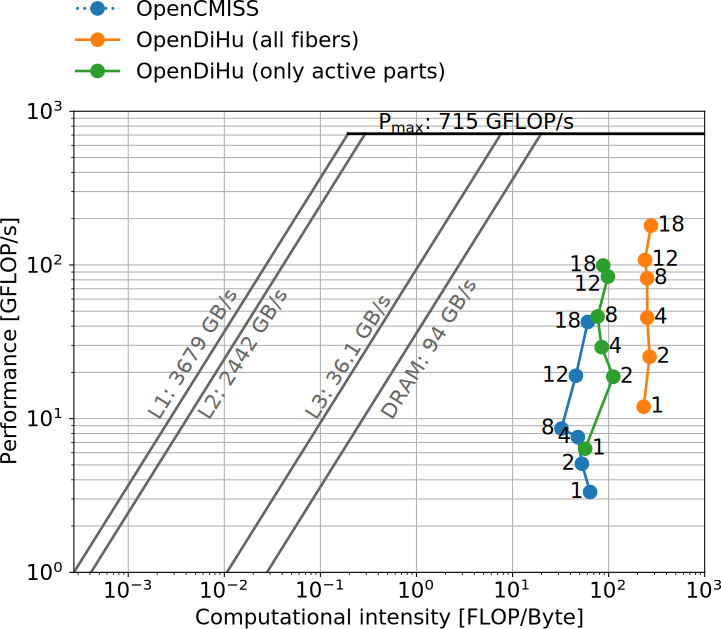
\includegraphics[width=\textwidth]{images/results/studies/0_roofline.pdf}%
  \caption{Roofline model}%
  \label{fig:roofline}%
\end{figure}%

%-----
\section{GPU}

\begin{figure}%
  \centering%
  \begin{subfigure}[t]{0.48\textwidth}%
    \centering%
    \includegraphics[height=6.5cm]{images/results/studies/16_hodgkin_huxley_gpu.png}%
    \caption{a.}%
    \label{fig:16_hodgkin_huxley_gpu}%
  \end{subfigure}
  \,
  \begin{subfigure}[t]{0.48\textwidth}%
    \centering%
    \includegraphics[height=6.5cm]{images/results/studies/16_hodgkin_huxley_cpu.png}%
    \caption{a.}%
    \label{fig:16_hodgkin_huxley_cpu}%
  \end{subfigure}   
  \caption{gpu.}%
  \label{fig:16_hodgkin_huxley_cpu_gpu}%
\end{figure}%

%-----
\section{Opendihu Weak scaling}
Hazel hen plot of coupled paper, new plots on hawk
% performance/opendihu/08_0D1D_better_implementation
%-----
\section{Opendihu rank placement strategies}

%-----
\section{Multidomain Solvers}

% linear solvers for multidomain
\begin{figure}[H]%
  \centering%
  \includegraphics[width=\textwidth]{images/results/studies/multidomain_solvers_all.png}%
  \caption{Caption}%
  \label{fig:fig1}%
\end{figure}
%-----
\section{Output file sizes}
%-----
%\section{Mesh convergence, stochastic with different MU assignments}
%-----
\section{dx-dt dependencies}
\section{Propagation velocity}

%performance/opendihu/03_dx_dt_dependence
%performance/opendihu/09_monodomain_dt0D_dt1D
%-----
\section{PinT}
%-----
\section{Load balancing}
%-----
\section{Application of opendihu within the field of robotics}

\chapter{Conclusion and Future Work}\label{sec:conclusion_and_future_work}

\section{Future Work}\label{sec:future_work}
 
% more timestepping methods: CVODE (https://computing.llnl.gov/projects/sundials/cvode), imex
% different parallelisation where not all ranks have to be involved (for multidomain) -> this feature already exists for the fibers with multipleInstances




